\begin{enunciado}{\ejercicio}
  Calcular los módulos y los argumentos de los siguiente números complejos
  Hallar todos los número complejos $z$ tales que
  \begin{multicols}{4}
    \begin{enumerate}[label=\roman*)]
      \item $(2+2i)(\sqrt{3} - i)$
      \item $(-1 + \sqrt{3}i)^5$
      \item $(-1 + \sqrt{3}i)^{-5}$
      \item $\displaystyle\frac{1+\sqrt{3}i}{1-i}$.
    \end{enumerate}
  \end{multicols}
\end{enunciado}

\begin{enumerate}[label=\roman*)]
  \item A mí me gusta usar propiedades de potencia para calcular la forma final del número:

        \begin{minipage}{0.2\textwidth}
          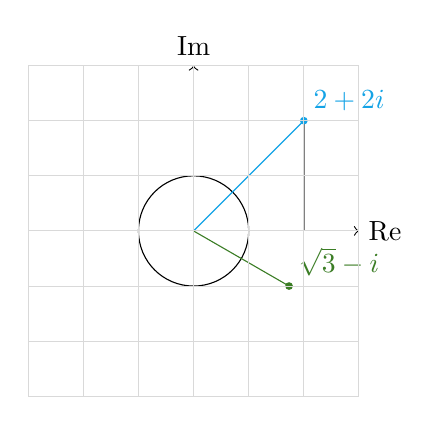
\begin{tikzpicture}[scale=0.7]
            % Draw dashed lines to axes
            \draw[help lines] (2,2) grid (2,0);
            % Draw the axes
            \draw[->] (-3,0) -- (3,0) node[right] {Re};
            \draw[->] (0,-3) -- (0,3) node[above] {Im};

            % Draw the unit circle
            \draw[thin] (0,0) circle (1);

            % Draw the point (2,2)
            \fill[Cerulean] (2,2) circle (2pt) node[above right] {$2+2i$};
            \fill[OliveGreen] ({sqrt(3)}, -1) circle (2pt) node[above right] {$\sqrt{3} - i$};

            % Draw the vector from origin to point
            \draw[Cerulean] (0,0) -- (2,2);
            \draw[OliveGreen] (0,0) -- ({sqrt(3)}, -1);

            % Add gridlines (optional)
            \draw[gray!30] (-3,-3) grid (3,3);
          \end{tikzpicture}
        \end{minipage}
        \begin{minipage}{0.7\textwidth}
          $$
            z = \blue{(2+2i)} \cdot \green{(\sqrt{3} - i)}
            \igual{\red{!}}
            \blue{2\sqrt{2}e^{i \frac{\pi}{4}}} \cdot \green{2 e^{i\frac{11}{6}\pi}}
          $$
        \end{minipage}

        Y ahora como se están multiplicando las potencias, solo hay que usar propiedades de potencias:

        $$
          z = 4\sqrt{2} e^{i\frac{25}{12}\pi}
        $$
        Recordar que el argumento por definición está en $[0, 2\pi)$, así que si es mayor o menos se le restan o suman $2k\pi$ respectivamente hasta que
        caiga en el intervalo.

        Por lo que el resultado pedido quedaría en:
        $$
          \cajaResultado{
            |z| = 4\sqrt{2}
            \ytext
            \arg(z) = \frac{1}{12} \pi
          }
        $$

  \item Como el anterior pero más fácil:

        \begin{minipage}{0.2\textwidth}
          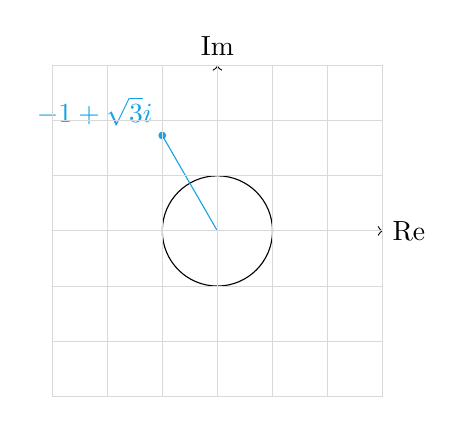
\begin{tikzpicture}[scale=0.7]
            % Draw dashed lines to axes
            \draw[help lines] (2,2) grid (2,0);
            % Draw the axes
            \draw[->] (-3,0) -- (3,0) node[right] {Re};
            \draw[->] (0,-3) -- (0,3) node[above] {Im};

            % Draw the unit circle
            \draw[thin] (0,0) circle (1);

            % Draw the point (2,2)
            \fill[Cerulean] (-1,{sqrt(3)}) circle (2pt) node[above left] {$-1+\sqrt{3}i$};

            % Draw the vector from origin to point
            \draw[Cerulean] (0,0) -- (-1,{sqrt(3)});

            % Add gridlines (optional)
            \draw[gray!30] (-3,-3) grid (3,3);
          \end{tikzpicture}
        \end{minipage}
        \begin{minipage}{0.7\textwidth}
          $$
            z = \blue{(-1 + \sqrt{3}i)^5}
            \igual{\red{!}}
            \blue{2^5 e^{i \frac{2}{3} \cdot 5\pi}}
            =
            \blue{32 e^{i \frac{10}{3} \pi}}
          $$
        \end{minipage}

        Nuevamente, corrijo el argumento para que caiga en el intervalo $[0, 2\pi)$.
        Por lo que el resultado pedido quedaría en:
        $$
          \cajaResultado{
            |z| = 32
            \ytext
            \arg(z) = \frac{4}{3} \pi
          }
        $$

  \item Parecido al anterior:
        $$
          z = \blue{(-1 + \sqrt{3}i)^{-5}}
          \igual{\red{!}}
          \blue{2^{-5} e^{i \frac{2}{3} \cdot (-5)\pi}}
          =
          \blue{\frac{1}{32} e^{-i \frac{10}{3} \pi}}
        $$

        Nuevamente, corrijo el argumento para que caiga en el intervalo $[0, 2\pi)$.
        Por lo que el resultado pedido quedaría en:
        $$
          \cajaResultado{
            |z| = \frac{1}{32}
            \ytext
            \arg(z) = \frac{2}{3} \pi
          }
        $$

  \item Parecido a lo anterior:

        \begin{minipage}{0.2\textwidth}
          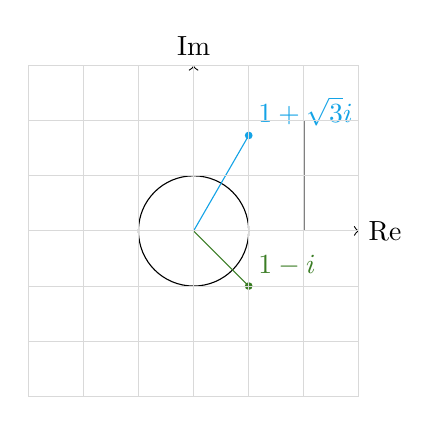
\begin{tikzpicture}[scale=0.7]
            % Draw dashed lines to axes
            \draw[help lines] (2,2) grid (2,0);
            % Draw the axes
            \draw[->] (-3,0) -- (3,0) node[right] {Re};
            \draw[->] (0,-3) -- (0,3) node[above] {Im};

            % Draw the unit circle
            \draw[thin] (0,0) circle (1);

            % Draw the point (2,2)
            \fill[Cerulean] (1,{sqrt(3)}) circle (2pt) node[above right] {$1 + \sqrt{3} i$};
            \fill[OliveGreen] (1, -1) circle (2pt) node[above right] {$1 - i$};

            % Draw the vector from origin to point
            \draw[Cerulean] (0,0) -- (1,{sqrt(3)});
            \draw[OliveGreen] (0,0) -- (1, -1);

            % Add gridlines (optional)
            \draw[gray!30] (-3,-3) grid (3,3);
          \end{tikzpicture}
        \end{minipage}
        \begin{minipage}{0.7\textwidth}
          $$
            z = \frac{\blue{1+\sqrt{3}i}}{\green{1 - i}}
            \igual{\red{!}}
            \frac{\blue{2 e^{i \frac{\pi}{3}}}}{\green{\sqrt{2} e^{i\frac{7}{4}\pi}}}
            =
            \sqrt{2}e^{-\frac{17}{12}\pi}
          $$
        \end{minipage}

        Recordar que el argumento por definición está en $[0, 2\pi)$, así que si es mayor o menos se le restan o suman $2k\pi$ respectivamente hasta que
        caiga en el intervalo.

        Por lo que el resultado pedido quedaría en:
        $$
          \cajaResultado{
            |z| = \sqrt{2}
            \ytext
            \arg(z) = \frac{7}{12} \pi
          }
        $$
\end{enumerate}

\begin{aportes}
  \item \aporte{\dirRepo}{Nad Garraz \github}
\end{aportes}
